\section{Introduction}
%Over the last decade how the CO2 levels have increased from 200 ppm to 400 ppm. 
%General overview of carbon emissions and climate accords.
It has come to the attention to most governmental bodies and general public that the threat of global warming is real. It is also noted that this year most countries recorded their highest ever temperature records for example, this year's July $25^{th}$ marked the hottest ever since the first recorded temperature at 1901 in the Netherlands \cite{Pieters2019}. According to Allen et al., the $CO_2$ emissions into the atmosphere is estimated to be over 3.67 trillion tones of $CO_2$, this will cause a carbon dioxide caused warming of 2 \degree C above the pre-industrial temperatures by 2500 \cite{Allen2009}. $CO_2$ direct air capture or DAC is growing interest in research and development in order to fight climate change. There is two types of DAC systems at the moment. High temperature solid sorbent (HT DAC) systems that operate at about 800 - 900 \degree C using carbonates or Sodium tri - titanante. The second type is low temperature solid (LT DAC) system that operate at temperature ranges from 80 to 120 \degree C using polyamines \cite{Fasihi2019}.

\subsection{Low temperature solution DAC}
\noindent
In order to address the growing concerns of carbon emissions and global warming. The people at Zero Emission Fuels B.V (ZEF) are trying to make a micro-plant that is capable of capturing $CO_2$ from the atmosphere and converting into industry grade (AA grade) methanol that can used as fuel or chemical feedstock. The plant is powered by photo-voltaic solar power which reduces the carbon footprint even more. The energy is utilized in the Alkaline electrolysis cell (AEC) that produces $H_2$, which reacts with $CO_2$ and makes methanol ($CH_{3}OH$) and to run the pumps and compressors across the micro-plant. At ZEF, we work with polyamines and hence, the DAC system used is a low temperature sorbent solution using PEI or TEPA. 

\begin{figure}[H]
    \centering
    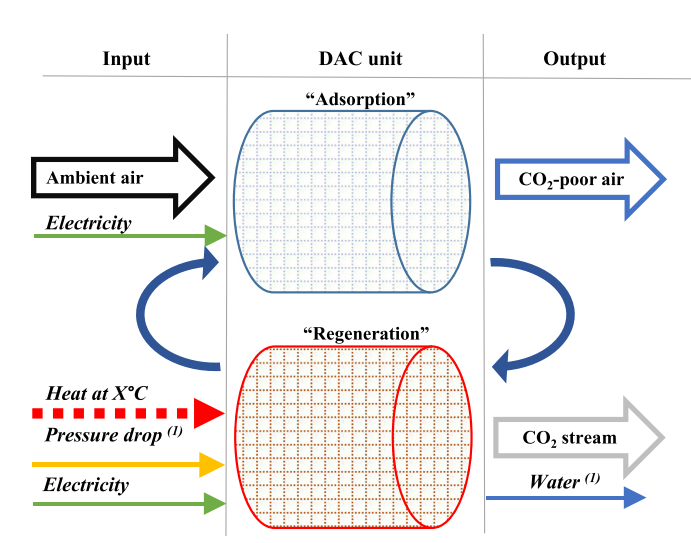
\includegraphics[scale = 0.6]{images/LT_DAC.png}
    \caption{Low temperature solution DAC system}
    \label{fig:LTDAC}
\end{figure}

\noindent
In Figure \ref{fig:LTDAC} above, an example of a LT DAC system can be seen and based on this model. Fasihi et al. talks about all kinds of DAC systems that are available at present and has given a economic analysis of each system based on DAC companies that are working at present such as Climeworks, Carbon Engineering, Antecy, etc. However, I shall limit the discussion to LT DAC systems as the DAC system that is present in ZEF is a LT DAC system. 


% Table generated by Excel2LaTeX from sheet 'Sheet1'
\begin{table}[htbp]
  \centering
  \caption{LT DAC specifications \cite{Fasihi2019}}
  \tiny{
    \begin{tabular}{|l|c|c|c|c|c|c|c|c|c|c|}
    \hline
    \textbf{Sorbent} & \textbf{$CO_2$ conc.} & \textbf{adsorption} & \multicolumn{2}{c|}{\textbf{desorption}} & \multicolumn{3}{c|}{\textbf{energy demand}} & \multicolumn{2}{c|}{\textbf{cooling }} & \textbf{$CO_{2}$ purity} \\
    \hline
          &       & T     & T     & P     &       &       & by    & T     &       &  \\
    \hline
       Units   & ppm   & \degree C & \degree C & bar   & $kWh_{el}/t$ & $kWh_{he}/t$ &       & \degree C &      & \%  \\
    \hline
    amine-based & 400   & ambient & 100   & 0.2   & 200-300 & 1500-2000 & waste heat & 15    & air/water & 99.9 \\
    \hline
    amino-polymer & 400   & ambient & 85-95  & 0.5-0.9 & 150-260 & 1170-1410 & steam & ambient & water evaporation & >98.5 \\
    \hline
    TRI-PE-MCM-41 & 400   & ambient & 110   & 1.4   & 218   & 1656  & steam & -    & -    & 88 \\
    \hline
    MOF (Cr) & 400   & ambient & 135-480 & 1     & 1420  &    -   & HT steam & -    & -    & - \\
    \hline
    MOF (MG) & 400   & ambient & 135-480 & 1     & 997   &    -   & HT steam  & -    & -    & - \\
    \hline
    $K_{2}CO_{3}$/$Y_{2}O_{3}$ & 400   & ambient & 150-250 & -    &    -   &    -   & el. Heater & -    & -    & - \\
    \hline
    $K_{2}CO_{3}$ & -    & ambient & 80-100 & -    & 694   & 2083  & waste heat & ambient & airflow & - \\
    \hline
    \end{tabular}%
    }
  \label{tab:ltdac}%
\end{table}%

\noindent
In Table \ref{tab:ltdac}, it can be seen that amine - based sorbent DAC systems has the maximum $CO_2$ purity based on literature \cite{Fasihi2019}. Compared to ZEF's competitors like Antecy in Netherlands and Climeworks in Switzerland, who use waste heat from industries to heat their desorption units and only store the carbon in these amines. ZEF has the upperhand and aim to bring the price down to 40 euros per ton of $CO_2$ captured by relying on solar energy to provide the process energy required to run the microplant. The cost is further brought down as ZEF conducts methanol synthesis using the absorbed $CO_2$ to AA grade methanol that can be used as alternative fuels. Thereby making it a completely carbon negative carbon capture utilization system. According to Fasihi et al., the cost of LT DAC systems can drop to potentially event 32 euros / ton of $CO_2$ in the year 2050. Unlike its DAC competitors who absorb $CO_2$ from high carbondioxide emission industries only, ZEF captures $CO_2$ directly from the atmosphere.  


\subsection{Report overview}

In this report we will see the scope of my internship and what I had done with my time at Zero Emission Fuels B.V. I cover a section on previous work done on the Direct Air Capture system in Zero Emission Fuels B.V that laid a foundation on what I should do and on what I should improve on in Section \ref{sec:prework}. In Section \ref{sec:mywork}, I cover what I did in the span of my internship. The internship was divided in the form of Sprints which is periods of 3 weeks, hence the whole internship contains 5 Sprints in total. I have described what I have done in each Sprint from Section \ref{sec:sprint1} to Section \ref{sec:sprint5}. In Section \ref{sec:results} contains the main observations made from running the DAC systems. Based on the findings from Section \ref{sec:results}, I have written the discussion of results in Section \ref{sec:results}. I have made some suggestions for the next Direct Air Capture team of ZEF VI in Section \ref{sec:recom} and added concluded the report in Section \ref{sec:conc}